\noindent
\begin{minipage}[t]{122pt}
  \vspace{0pt}
  % CỘT LỀ TRÁI: Dóng hàng chính xác theo tọa độ y của bản gốc
  \vspace{158pt}
  
  % Hộp ghi chú Problem Solving (y=223.1pt)
  \begin{tcolorbox}[
      colback=psboxbg,
      colframe=pspurple!25,
      arc=1mm,
      boxrule=0.4pt,
      left=3pt,
      right=3pt,
      top=3pt,
      bottom=3pt
  ]
  \noindent\colorbox{pspurple}{\textcolor{white}{\fontsize{6}{7}\selectfont\textbf{\textsf{PS}}}}\hspace{2pt}%
  \fontsize{7.5}{9.5}\selectfont
  Giai đoạn thứ hai của việc giải toán là suy nghĩ một kế hoạch để kết nối dữ kiện đã cho và đại lượng cần tìm.
  \end{tcolorbox}

  % Lưu ý dV/dt (y=300.4pt)
  \vspace{44pt}
  {\fontsize{7.5}{9.5}\selectfont\noindent Lưu ý rằng, mặc dù $dV/dt$ là hằng số, nhưng $dr/dt$ \emph{không} phải là hằng số.\par}

  % Hình 1 (y=401.6pt - dóng ngang đầu Ví dụ 2)
  \vspace{82pt}
  \centering
  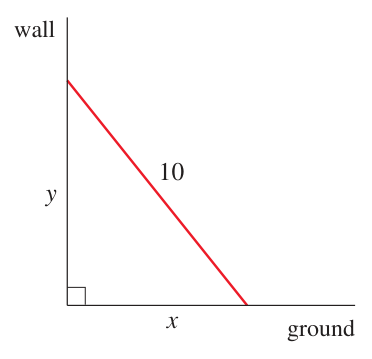
\includegraphics[width=\linewidth]{images/p0283_fig1.png}
  \vspace{3pt}
  {\fontsize{8}{10}\selectfont\textbf{\textsf{HÌNH 1}}\par}

  % Hình 2 (y=550.0pt - dóng ngang biểu thức đạo hàm chuỗi)
  \vspace{27pt}
  \centering
  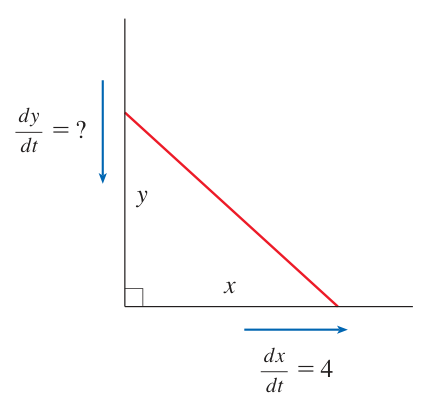
\includegraphics[width=\linewidth]{images/p0283_fig2.png}
  \vspace{3pt}
  {\fontsize{8}{10}\selectfont\textbf{\textsf{HÌNH 2}}\par}
\end{minipage}%
\hspace{22pt}%
\begin{minipage}[t]{360pt}
  \vspace{0pt}
  % CỘT NỘI DUNG CHÍNH
  \fontsize{9.5}{13}\selectfont
  Điều cốt lõi cần nhớ là các tốc độ thay đổi chính là đạo hàm. Trong bài toán này, thể tích và bán kính đều là các hàm số theo thời gian $t$. Tốc độ tăng của thể tích theo thời gian là đạo hàm $dV/dt$, và tốc độ tăng của bán kính là $dr/dt$. Do đó, ta có thể phát biểu lại đại lượng đã cho và đại lượng chưa biết như sau:
  
  \vspace{4pt}
  \begin{center}
  \renewcommand{\arraystretch}{1.3}
  \begin{tabular}{ll}
      \textit{Đã cho:} & $\dfrac{dV}{dt} = 100\text{ cm}^3/\text{s}$ \\[8pt]
      \textit{Cần tìm:} & $\dfrac{dr}{dt}\quad\text{khi } r = 25\text{ cm}$
  \end{tabular}
  \end{center}
  \vspace{3pt}

  Để kết nối $dV/dt$ và $dr/dt$, trước tiên ta liên hệ $V$ và $r$ bằng một công thức---trong trường hợp này là công thức tính thể tích của hình cầu:
  \[
  V = \frac{4}{3}\pi r^3
  \]
  Để sử dụng thông tin đã cho, ta lấy đạo hàm hai vế của phương trình này theo $t$. Để lấy đạo hàm vế phải, ta cần dùng Quy tắc chuỗi:
  \[
  \frac{dV}{dt} = \frac{dV}{dr} \frac{dr}{dt} = 4\pi r^2 \frac{dr}{dt}
  \]
  Bây giờ ta giải phương trình để tìm đại lượng chưa biết:
  \[
  \frac{dr}{dt} = \frac{1}{4\pi r^2} \frac{dV}{dt}
  \]
  Nếu thay $r = 25$ và $dV/dt = 100$ vào phương trình này, ta nhận được
  \[
  \frac{dr}{dt} = \frac{1}{4\pi (25)^2} 100 = \frac{1}{25\pi}
  \]
  Bán kính của quả bóng đang tăng với tốc độ $1/(25\pi) \approx 0{,}0127\text{ cm/s}$ khi đường kính bằng $50\text{ cm}$.\hfill{\color{stewartcyan}\rule{1.1ex}{1.1ex}}

  \vspace{10pt}
  \noindent\textbf{\textsf{\color{stewartcyan}VÍ DỤ 2}}\hspace{0.8em}Một chiếc thang dài $10\text{ ft}$ tựa vào một bức tường thẳng đứng. Nếu chân thang trượt ra xa tường với tốc độ $4\text{ ft/s}$, thì đỉnh thang trượt xuống dọc theo bức tường với tốc độ bao nhiêu khi chân thang cách tường $6\text{ ft}$?

  \vspace{5pt}
  \noindent\textbf{\textsf{\color{stewartcyan}LỜI GIẢI}}\hspace{0.8em}Trước tiên ta vẽ một sơ đồ và đặt tên các biến như trong Hình 1. Gọi $x$ feet là khoảng cách từ chân thang đến tường và $y$ feet là khoảng cách từ đỉnh thang đến mặt đất. Chú ý rằng cả $x$ và $y$ đều là các hàm số theo $t$ (thời gian, tính bằng giây).

  \vspace{3pt}
  Ta đã biết $dx/dt = 4\text{ ft/s}$ và cần tìm $dy/dt$ khi $x = 6\text{ ft}$ (xem Hình 2). Trong bài toán này, mối liên hệ giữa $x$ và $y$ được xác định bởi Định lý Pytago:
  \[
  x^2 + y^2 = 100
  \]
  Lấy đạo hàm hai vế theo $t$ bằng cách sử dụng Quy tắc chuỗi, ta có
  \[
  2x \frac{dx}{dt} + 2y \frac{dy}{dt} = 0
  \]
  Giải phương trình này để tìm tốc độ cần tính, ta được
  \[
  \frac{dy}{dt} = -\frac{x}{y}\frac{dx}{dt}
  \]
  Khi $x = 6$, Định lý Pytago cho ta $y = 8$, và vì thế, thay các giá trị này cùng với $dx/dt = 4$, ta có
  \[
  \frac{dy}{dt} = -\frac{6}{8}(4) = -3\text{ ft/s}
  \]
\end{minipage}
